\usetikzlibrary{shapes,arrows,chains}
\usetikzlibrary[calc]
\usetikzlibrary{shapes.geometric, arrows, fit, calc, automata, positioning, shapes.multipart}
\usepackage{comment}
\renewenvironment{comment}{}{}
    %%% done
    % Events
    \tikzstyle{arrow} = [thick,->,>=stealth]

    \tikzstyle{state} = [rectangle, minimum width=1.5cm, minimum height=1cm, text centered, draw=black, fill=white!30]

    \tikzstyle{cluster} = [line width=0.4pt, draw=black, inner sep=0.5em, rounded corners=0.1cm]

    \usetikzlibrary{shapes.geometric, arrows, fit, calc, automata, positioning}
\tikzstyle{umlcolor}=[
    color=\umldrawcolor,
    fill=\umlfillcolor,
    text=\umltextcolor
]
\tikzstyle{umlcd style class}=[
    draw,
    rectangle,
    rectangle split,
    rectangle split parts=3,
    rounded corners,
    text centered,
    text height=1em,
    text width=2.2cm,
    text depth = 0.5em,
    fill=white
]
\tikzstyle{event_start} = [draw,circle,scale=.30,fill=black]
\tikzset{
  event_end/.style={
    label={[draw,circle,scale=1.3,fill=white,line width=0.4mm]center:},
    label={[draw,circle,scale=.75,fill=black]center:}
  }
}
\tikzstyle{block} = [rectangle, draw, text width=6em, text centered, rounded corners, minimum height=4em]
\tikzstyle{line} = [draw, -latex']

\section{ML Pipeline}
When working with machine learning, pipelines helps to understand the different steps involved in the process. The following figure \ref{fig:ml-pipeline} shows the different steps that are involved in the process of building a machine learning model.
ML pipelines are usually divided into three main steps: data, feature extraction, model training and model evaluation. The following sections will describe each of these steps in more detail. 

In the figure \ref{fig:ml-pipeline} the box with the name "data" is representing the input to the machine learning pipeline. The data can be in different formats, such as images, text, audio, video, etc. The data is usually stored in a database or in a file. This is also the step data cleaning is done, which is the process of removing or replacing missing values in the data. In this step the data is processed into a format that can be used by the machine learning algorithm by for example taking data out a picture. 

Feature extraction (in \ref{fig:ml-pipeline} FE) is the process of extracting features from the data. This is done by for example dimensionality reduction or labelling correlated data, that is clustered together after the feature extraction. There are different methods that can be used on feature extraction, the ones used in the project will be discussed in another section \ref{sec:NOT_MADE_YET}. After going through the feature extraction the data os now ready to be out into a ML  model.
\begin{figure}
\centering
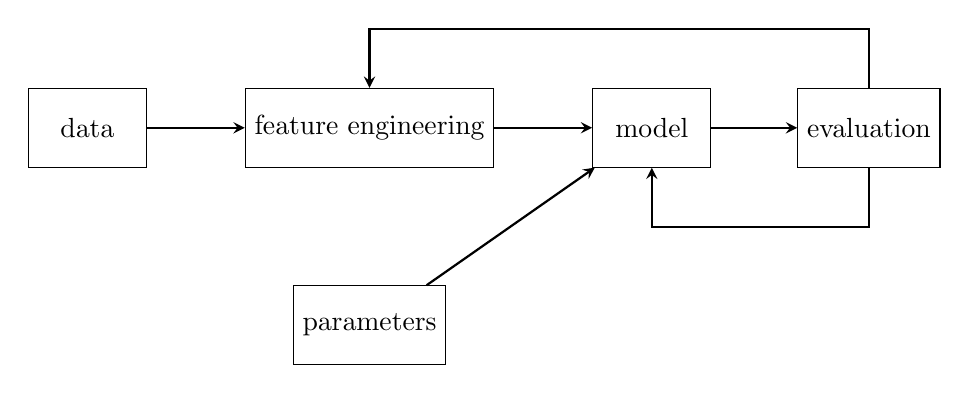
\begin{tikzpicture}
	\node (b) [state] {feature engineering};
	\node (c) [state,shift={($(b.east)+(2cm,0)$)}] {model};
	\node (a) [state, shift={($(b.west)+(-2cm,0)$)}] {data};
	\node (d) [state,shift={($(c.east)+(2cm,0)$)}] {evaluation};
	\node (e) [state, shift={($(b.south)+(0,-2cm)$)}] {parameters};
	
	\draw[arrow, ->] (a) -- node[above,scale=.70,align=center,] {} (b);
	\draw[arrow, ->] (b) -- node[above,scale=.70,align=center,] {} (c);
	\draw[arrow, ->] (c) -- node[above,scale=.70,align=center,] {} (d);
    \draw[arrow, ->] (e) -- node[above,scale=.70,align=center,] {} (c);

    \draw [arrow, ->] (d.north) -- ++(0,0.75) -| (b);
    \draw [arrow, ->] (d.south) -- ++(0,-0.75) -| (c);
\end{tikzpicture}          
\caption{ML pipeline}
\label{fig:ml-pipeline}
\end{figure}

The box "parameters" in figure \ref{fig:ml-pipeline} describes the parameters that are used in the model. The parameters are the values that are used to train the model. The parameters are usually set by the user, but can also be set by the model itself. The parameters uses various metrics such as accuracy, precision, speed and memory usage to detemain if the model is the correct fit. To see if the model is good fit, the model is evaluated in the evaluation stage. 

Model training is the process of training the model with the data. This is done by using a training set and a validation set. The training set is used to train the model to predict the output with highest possible accuracy. The validation set is used to evaluate the model. It is here where the chosen parameters determine the fit of the model. 
Model evaluation is the process for analysing the models performance. This is done by using a test set. The test set is used to evaluate the model. The test set is not used to train the model. The evaluation is done by comparing the predicted values with the actual values that was to be expected. After the model has been evaluated, new models or feature extraction can be used to try and improve the models performance \cite{ml_pipeline_javapoint}.


\begin{comment}   
@misc{ml_pipeline_javapoint,
  organization = {javapoint},
  url          = {https://www.javatpoint.com/machine-learning-pipeline},
  title        = {Machine Learning Pipeline},
  urldate      = {2022-10-04}
}
\end{comment}